\documentclass[12pt, a4paper]{article}
\usepackage{enumitem}
\usepackage{float}
\usepackage[left=2cm, right=2cm, top=2cm, bottom=2cm]{geometry}
\usepackage{graphicx}
\usepackage[colorlinks, urlcolor=blue]{hyperref}
\usepackage{minted}
\usepackage[table]{xcolor}
\usepackage{xeCJK}

\renewcommand\arraystretch{1.1}
\setCJKmainfont[AutoFakeBold=1.5]{新細明體}

\setminted{
  frame=single,
  framesep=4pt,
}

\title{
  Network Administration/System Administration\\
  (NTU CSIE, Spring 2024)\\
  Homework \#5 - Virsh, Docker \& Kubernetes
}
\author{\Large B12902110 呂承諺}

\begin{document}
  \maketitle
  \section*{Virsh}
  \begin{enumerate}
    \item \textbf{Command}
    \begin{Verbatim}[frame=single]
virt-install \
  --name b12902110 \
  --vcpus 8 \
  --memory 8192 \
  --disk /tmp2/b12902110/nasahw5/ubuntu.qcow2,format=qcow2,size=20 \
  --network user,mac=52:54:00:90:21:10 \
  --graphics type=vnc,password=902110,port=5950,listen=0.0.0.0 \
  --cdrom /tmp2/nasa-hw5/ubuntu.iso
    \end{Verbatim}

    \textbf{Result}

    \verb|virsh list|:

    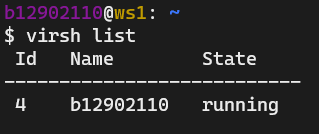
\includegraphics[width=0.3\textwidth]{1-1_virsh_list.png}

    After boot up:

    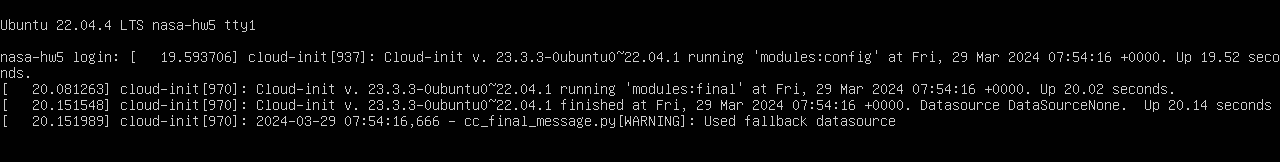
\includegraphics[width=0.93\textwidth]{1-1_boot.png}

    \pagebreak
    After login:

    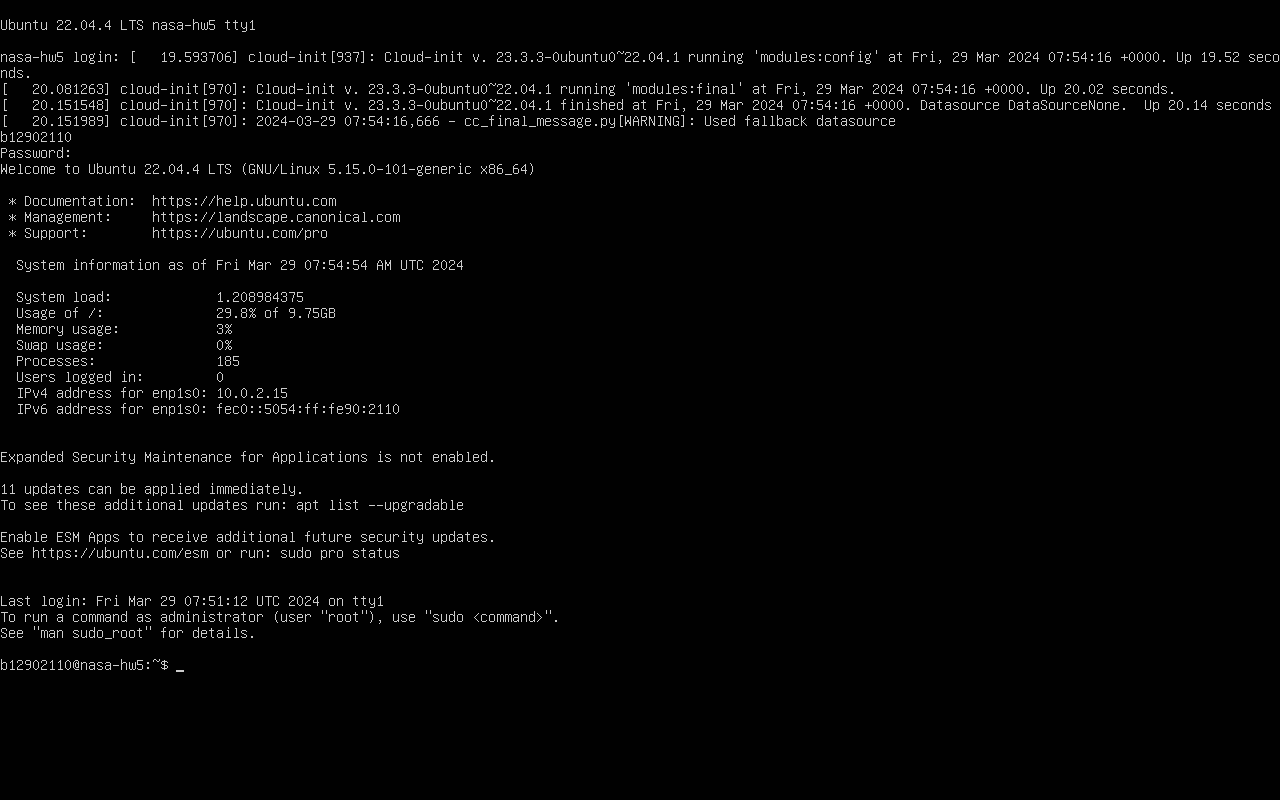
\includegraphics[width=0.93\textwidth]{1-1_login.png}

    \verb|ip a|:

    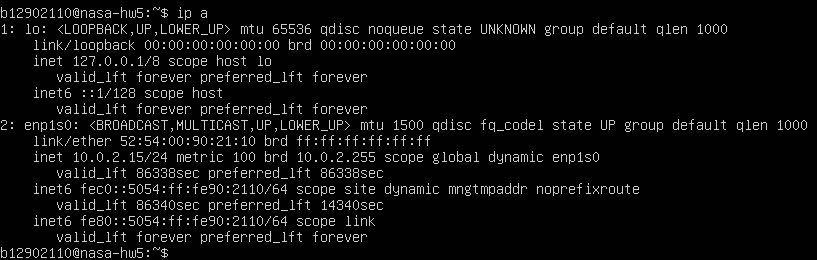
\includegraphics[width=0.93\textwidth]{1-1_ip_a.png}

    \item \textbf{Command (on VM)}
    \begin{minted}{shell}
sudo systemctl enable --now serial-getty@ttyS0.service
sudo systemctl enable --now ssh.service
    \end{minted}

    \textbf{Command (on host)}
    \begin{minted}{shell}
virsh qemu-monitor-command b12902110 --hmp 'hostfwd_add ::11022-:22'
    \end{minted}

    \pagebreak
    \textbf{Result}

    \begin{minipage}[t]{0.47\textwidth}
      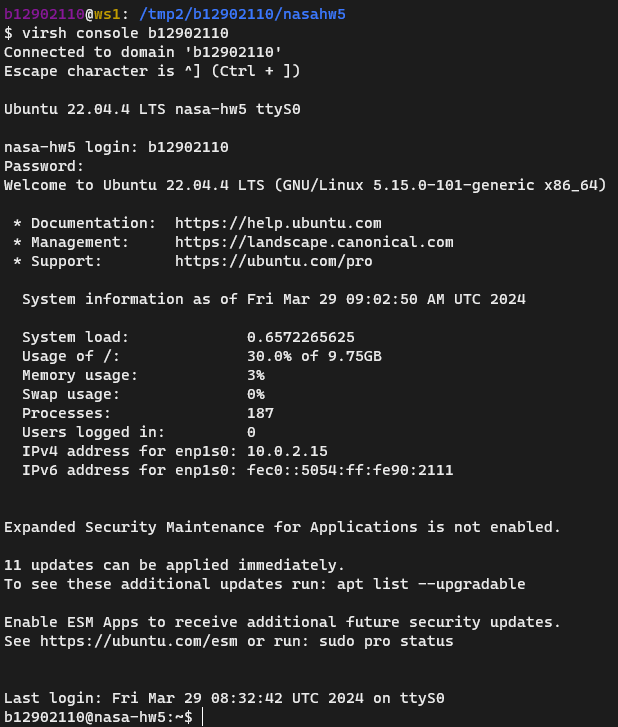
\includegraphics[width=\textwidth]{1-2_virsh_console.png}
    \end{minipage}
    \begin{minipage}[t]{0.48\textwidth}
      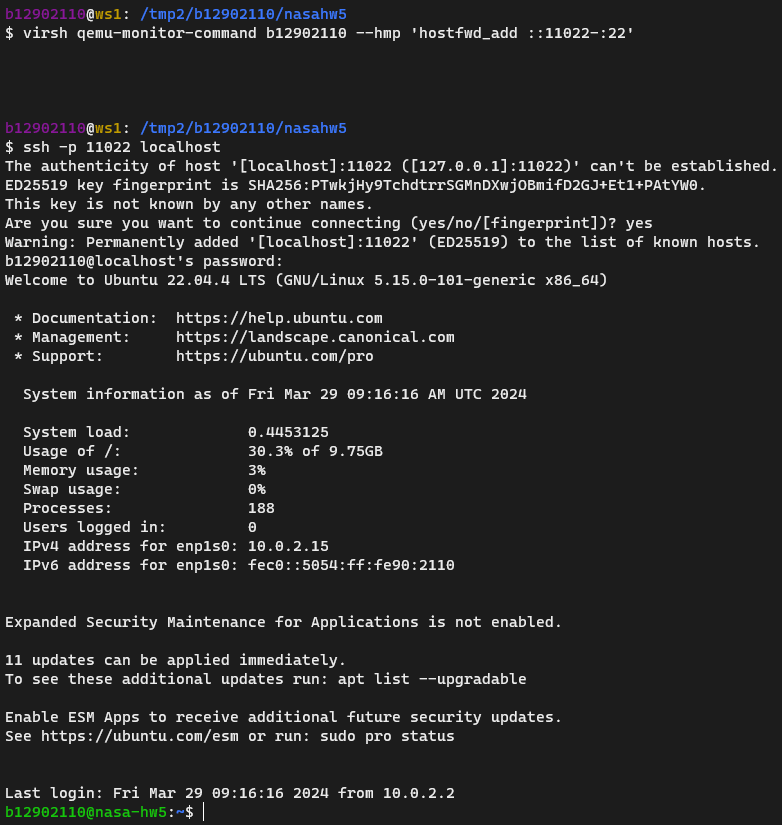
\includegraphics[width=\textwidth]{1-2_ssh.png}
    \end{minipage}
  \end{enumerate}

  \textbf{References}
  \begin{itemize}
    \item \verb|man virt-install|, \verb|man virsh|
      \item \href{https://libvirt.org/formatnetwork.html}{libvirt: Network XML format}
      \item \href{https://wiki.libvirt.org/TaskNATSetupVirtManager.html}{libvirt: Creating a NAT Virtual Network}
      \item \href{https://wiki.libvirt.org/Networking.html#host-configuration-nat}{libvirt: NAT forwarding (aka "virtual networks")}
      \item \href{https://libvirt.org/formatdomain.html}{libvirt: Domain XML format}
      \item \href{https://unix.stackexchange.com/questions/350339/how-to-port-forward-ssh-in-virt-manager}{qemu - How to port forward SSH in virt-manager? - Unix \& Linux Stack Exchange}
      \item \href{https://www.qemu.org/docs/master/system/invocation.html}{Invocation — QEMU  documentation}
      \item \href{https://serverfault.com/questions/890520/host-port-forward-with-qemu-through-libvirt-in-user-mode-networking}{host port forward with qemu through libvirt in user-mode networking - Server Fault}
      \item \href{https://blog.adamspiers.org/2012/01/23/port-redirection-from-kvm-host-to-guest/}{Structured Procrastination port redirection from kvm host to guest – Structured Procrastination}
  \end{itemize}

  \pagebreak
  \section*{Docker}
  \subsection*{Set Up}
  \begin{enumerate}[resume]
    \item \textbf{Command}
    \begin{minted}[fontsize=\footnotesize]{shell}
# Add Docker's official GPG key:
sudo curl -fsSL https://download.docker.com/linux/ubuntu/gpg \
  -o /etc/apt/keyrings/docker.asc
sudo chmod a+r /etc/apt/keyrings/docker.asc

# Add the repository to Apt sources:
# Add the repository to Apt sources:
echo \
  "deb [arch=$(dpkg --print-architecture) signed-by=/etc/apt/keyrings/docker.asc] \
  https://download.docker.com/linux/ubuntu \
  $(. /etc/os-release && echo "$VERSION_CODENAME") stable" | \
  sudo tee /etc/apt/sources.list.d/docker.list > /dev/null
sudo apt-get update

# Install the Docker packages.
sudo apt-get install docker-ce docker-ce-cli containerd.io docker-buildx-plugin \
  docker-compose-plugin docker-compose
    \end{minted}

   \textbf{Result}

   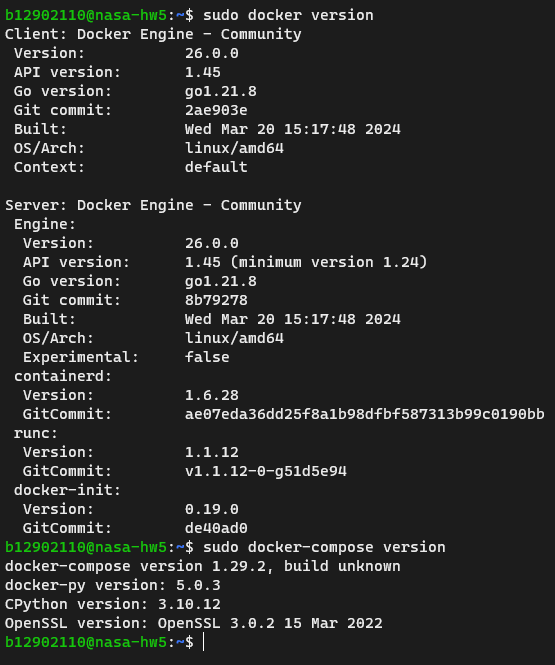
\includegraphics[width=0.45\textwidth]{2-1_docker_version.png}
  \end{enumerate}

  \subsection*{Docker Basics}
  \begin{enumerate}[resume]
    \item Cases to use Docker:
    \begin{itemize}
      \item Host OS is Linux.
      \item Application runs on Linux.
      \item When performance and efficiency is important, because Docker shares
      resources with the host.
      \item When we want to deploy the environment elsewhere, Docker offers better portability.
    \end{itemize}

    Cases to use VM:
    \begin{itemize}
      \item Host OS is not Linux.
      \item Application doesn't run on Linux.
      \item Need control over hardware resources (CPU, memory, etc.).
    \end{itemize}

    \textbf{References}
    \begin{itemize}
      \item \href{https://aws.amazon.com/compare/the-difference-between-docker-vm/}{Docker vs VM - Difference Between Application Deployment Technologies - AWS}
      \item \href{https://www.reddit.com/r/docker/comments/q6ykxa/when_should_you_choose_vms_over_docker/}{Reddit - Dive into anything}
    \end{itemize}

    \item The Docker Engine runs on a Linux kernel. On Windows and macOS, Docker
    is run in a virtual machine (WSL2 or LinuxKit VM), which hurts performance.

    \textbf{References}
    \begin{itemize}
      \item \href{https://www.usenimbus.com/post/instantly-improve-docker-performance-on-mac}{Instantly Improve Docker Performance on Mac}
      \item \href{https://www.cncf.io/blog/2023/02/02/docker-on-macos-is-slow-and-how-to-fix-it/}{Docker on MacOS is slow and how to fix it | CNCF}
      \item \href{https://docs.docker.com/desktop/install/windows-install/}{Install Docker Desktop on Windows | Docker Docs}
    \end{itemize}

    \item
    \begin{enumerate}
      \item \mintinline{shell}|docker stop $(docker ps -a -q)|

      ``\mintinline{shell}|docker ps -a -q|" list IDs of all containers.
      Substitute it into argument of ``\mintinline{shell}|docker stop|".

      \item \mintinline{shell}|docker image rm $(docker image -a -q)|

      ``\mintinline{shell}|docker image -a -q|" list IDs of all images.
      Substitute it into argument of\\ ``\mintinline{shell}|docker image rm|".

      \item \mintinline{shell}|docker system prune|

      Remove all unused containers, networks, images (both dangling and unused), and optionally, volumes.

      \item \phantom{}\vspace{-\baselineskip}

      \begin{minted}[fontsize=\footnotesize]{shell}
docker inspect \
  --format='{{range .NetworkSettings.Networks}}{{.IPAddress}}{{end}}' \
  5b0f1ed0dcb8
      \end{minted}

      Return low-level information on Docker objects.

      \item \mintinline{shell}|docker container stats|

      Display a live stream of container(s) resource usage statistics.
    \end{enumerate}

    \textbf{References}
    \begin{itemize}
      \item \href{https://stackoverflow.com/questions/45357771/stop-and-remove-all-docker-containers}{Stop and remove all docker containers - Stack Overflow}
      \item \href{https://docs.docker.com/reference/cli/docker/system/prune/}{docker system prune | Docker Docs}
      \item \href{https://stackoverflow.com/questions/17157721/how-to-get-a-docker-containers-ip-address-from-the-host}{How to get a Docker container's IP address from the host - Stack Overflow}
      \item \href{https://docs.docker.com/reference/cli/docker/inspect/}{docker inspect | Docker Docs}
      \item \href{https://docs.docker.com/reference/cli/docker/container/stats/}{docker container stats | Docker Docs}
    \end{itemize}

    \pagebreak
    \item
    \textbf{Command} \verb|docker run --name nginx-1 -d -p 8763:80 nginx:1.24.0|
    \begin{itemize}
      \item \verb|docker run|: Create and run a new container from an image.
      \item \verb|--name nginx-1|: Assign name \texttt{nginx-1} to container.
      \item \verb|-d|: Run in background.
      \item \verb|-p 8763 80|: Forward port 8763 on host to port 80 in container.
      \item \verb|nginx:1.24.0|: Image to run.
    \end{itemize}

    \textbf{Result}

    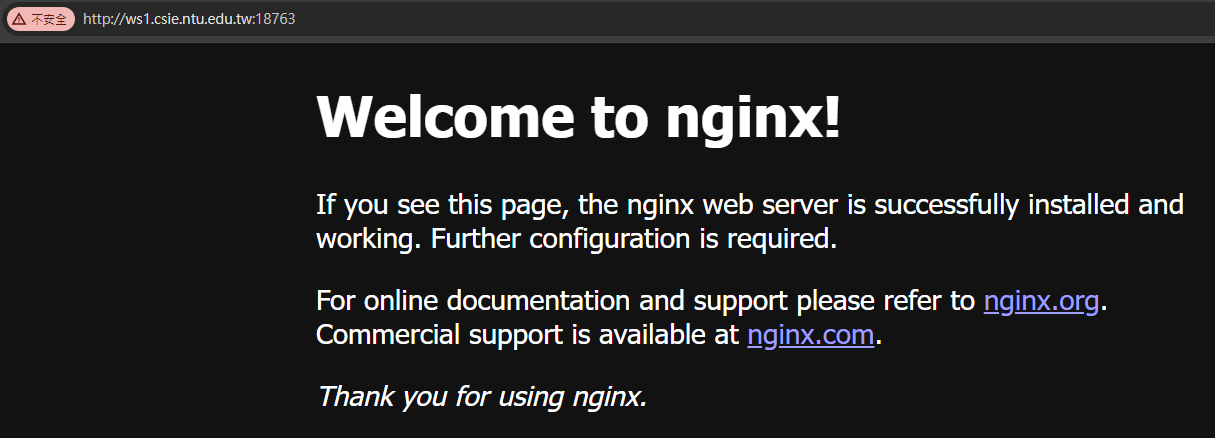
\includegraphics[width=0.9\textwidth]{7_nginx.png}

    Note: Port 18763 on ws1 is forwarded to port 8763 on Ubuntu VM.

    \textbf{References}
    \begin{itemize}
      \item \verb|docker run --help|
    \end{itemize}

    \item
    \textbf{Command} \verb|docker exec -it nginx-1 /bin/bash|
    \begin{itemize}
      \item \verb|docker exec|: Execute a command in a running container.
      \item \verb|-i|: Keep STDIN open even if not attached.
      \item \verb|-t|: Allocate a pseudo-TTY.
      \item \verb|nginx-1|: Container name.
      \item \verb|/bin/bash|: Command to execute.
    \end{itemize}

    \textbf{Result}

    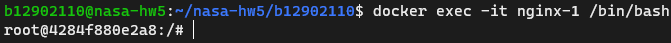
\includegraphics[width=0.9\textwidth]{8_docker_exec.png}

    \textbf{References}
    \begin{itemize}
      \item \verb|docker exec --help|
    \end{itemize}


    \pagebreak
    \item \textbf{Command} \verb|docker exec nginx-1 cat /etc/nginx/nginx.conf|

    \textbf{Result}

    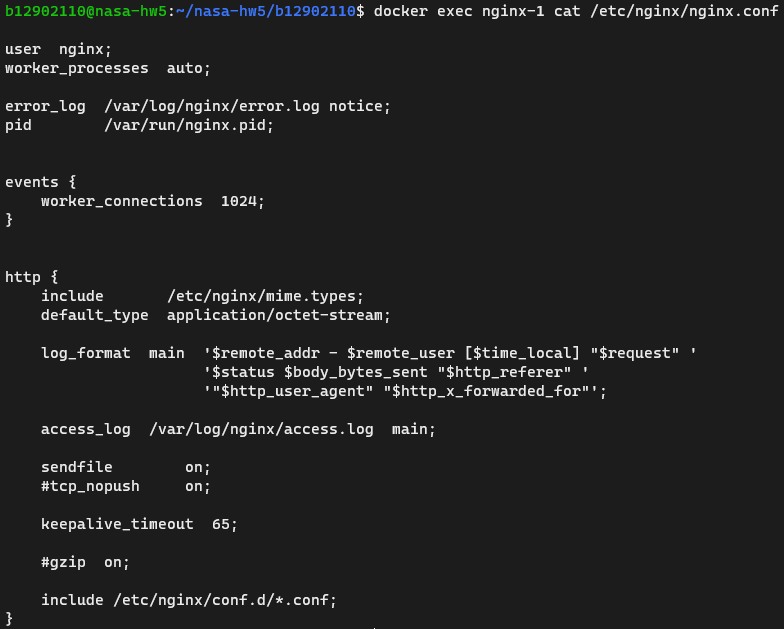
\includegraphics[width=0.7\textwidth]{9_docker_exec.png}

    \item
    \begin{enumerate}
      \item \verb|ENTRYPOINT| defines the executable that the container runs,
      \verb|CMD| defines default arguments for \verb|ENTRYPOINT|.
      \item \verb|ENTRYPOINT| is overridden with
      \verb|docker run --entrypoint NEW_ENTRY_POINT ...|.\\
      \verb|CMD| is overridden with \verb|docker run ... NEW_COMMAND|.
      \item If using exec form, \verb|CMD| is the arguments for \verb|ENTRYPOINT|.
    \end{enumerate}

    \textbf{References}
    \begin{itemize}
      \item \href{https://docs.docker.com/reference/dockerfile/}{Dockerfile reference | Docker Docs}
    \end{itemize}

    \item Docker Compose is a tool to manage \textit{multi-container} applications.
    We define services, network, volumes to be used in an YAML configuration file.
    On the other hand, Docker is the underlying virtualization engine that
    handles containers, images, networks, etc.

    \textbf{References}
    \begin{itemize}
      \item \href{https://docs.docker.com/engine/}{Docker Engine overview | Docker Docs}
      \item \href{https://docs.docker.com/compose/}{Docker Compose overview | Docker Docs}
    \end{itemize}

    \item
    \begin{enumerate}
      \item \textbf{Command} \verb|docker-compose up -d|
      \begin{itemize}
        \item \verb|docker-compose up|: Builds, (re)creates, starts, and attaches to containers for a service.
        \item \verb|-d|: Detached mode: Run containers in the background.
      \end{itemize}

      \item \textbf{Command} \verb|docker-compose pause|

      Pause services.

      \item \textbf{Command} \verb|docker-compose down -v|
      \begin{itemize}
        \item \verb|docker-compose down|: Stops containers and removes containers, networks, volumes, and images created by `up`.
        \item \verb|-v|: Remove volumes.
      \end{itemize}

    \end{enumerate}

    \textbf{References}
    \begin{itemize}
      \item \verb|docker-compose --help|
      \item \verb|docker-compose up --help|
      \item \verb|docker-compose pause --help|
      \item \verb|docker-compose down --help|
    \end{itemize}
  \end{enumerate}

  \subsection*{Application}
  \begin{enumerate}[resume]
    \item
    \textbf{b12902110.Dockerfile}
    \inputminted{docker}{b12902110/b12902110.Dockerfile}

    \textbf{Command}
    \begin{minted}{shell}
sudo docker build -t sl - < b12902110.Dockerfile
sudo docker run -it --rm sl
    \end{minted}

    \textbf{Result}

    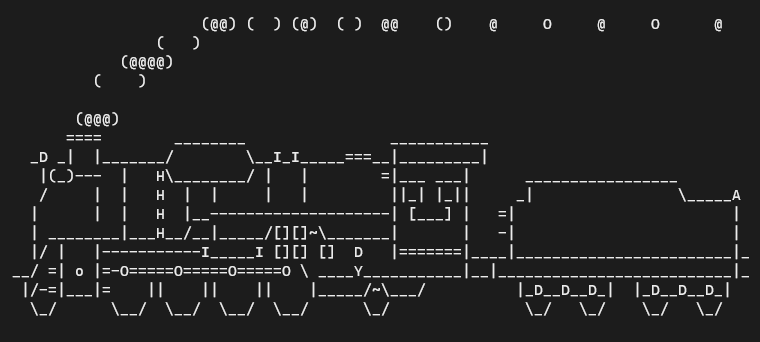
\includegraphics[width=0.4\textheight]{13_train.png}

    \textbf{References}
    \begin{itemize}
      \item \href{https://hub.docker.com/_/alpine}{alpine - Official Image | Docker Hub}
      \item \href{https://wiki.alpinelinux.org/wiki/Alpine_Package_Keeper}{Alpine Package Keeper - Alpine Linux}
      \item \href{https://wiki.alpinelinux.org/wiki/GCC}{GCC - Alpine Linux}
      \item \href{https://pkgs.alpinelinux.org/package/edge/main/x86_64/build-base}{Alpine Linux packages - build-base}
      \item \href{https://pkgs.alpinelinux.org/package/edge/main/x86_64/git}{Alpine Linux packages - git}
      \item \href{https://pkgs.alpinelinux.org/package/edge/main/x86_64/ncurses-dev}{Alpine Linux packages - ncurses-dev}
      \item \href{https://docs.docker.com/reference/dockerfile/}{Dockerfile reference | Docker Docs}
      \item \href{https://docs.docker.com/reference/cli/docker/image/build/}{docker build | Docker Docs}
    \end{itemize}

    \pagebreak
    \item
    \textbf{mysql-b12902110.yaml}
    \inputminted[fontsize=\footnotesize]{yaml}{b12902110/mysql-b12902110.yaml}

    \textbf{Command}
    \begin{minted}{shell}
sudo docker-compose -f mysql-b12902110.yaml up
    \end{minted}

    \textbf{Result}

    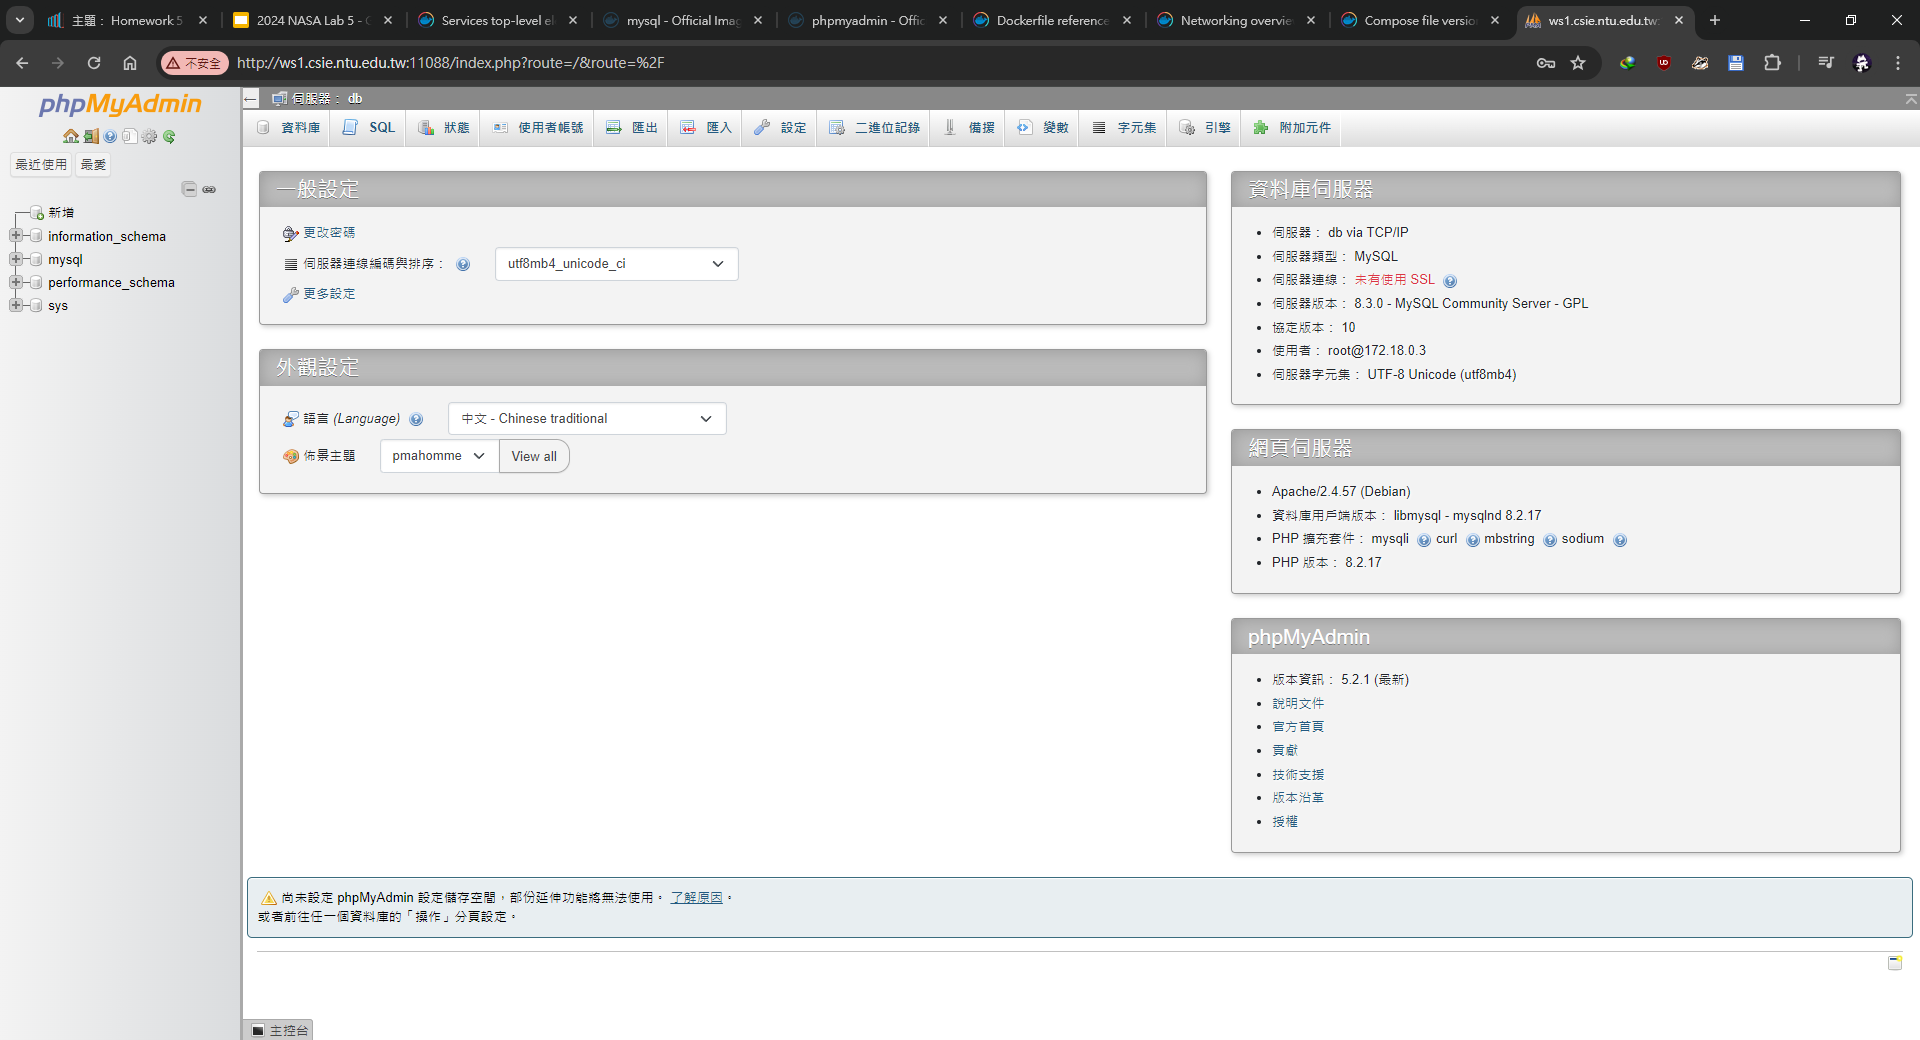
\includegraphics[width=0.93\textwidth]{14_phpmyadmin.png}
  \end{enumerate}

  \textbf{References}
  \begin{itemize}
    \item \href{https://docs.docker.com/compose/gettingstarted/}{Try Docker Compose | Docker Docs}
    \item \href{https://docs.docker.com/compose/networking/}{Networking in Compose | Docker Docs}
    \item \href{https://hub.docker.com/_/mysql}{mysql - Official Image | Docker Hub}
    \item \href{https://hub.docker.com/_/phpmyadmin}{phpmyadmin - Official Image | Docker Hub}
    \item \href{https://dev.mysql.com/doc/refman/5.7/en/environment-variables.html}{MySQL :: MySQL 5.7 Reference Manual :: 4.9 Environment Variables}
    \item \href{https://docs.docker.com/compose/environment-variables/set-environment-variables/}{Ways to set environment variables with Compose | Docker Docs}
  \end{itemize}

  \section*{Kubernetes}
  \begin{enumerate}[resume]
    \item
    \item
    \begin{enumerate}
      \item
      \textbf{Steps}
      \begin{enumerate}
        \item Reuse the VM installed in step 1.
        \item Run the following commands:
        \begin{minted}[fontsize=\scriptsize]{shell}
curl -LO https://storage.googleapis.com/minikube/releases/latest/minikube-linux-amd64
sudo install minikube-linux-amd64 /usr/local/bin/minikube && rm minikube-linux-amd64
alias kubectl="minikube kubectl --"
kubectl
        \end{minted}
      \end{enumerate}
      \item
      \textbf{nginx-b12902110.yaml}
      \inputminted[fontsize=\footnotesize]{yaml}{nginx-b12902110.yaml}
      \textbf{mysql-b12902110.yaml}
      \inputminted[fontsize=\footnotesize]{yaml}{mysql-b12902110.yaml}
      \textbf{phpmyadmin-b12902110.yaml}
      \inputminted[fontsize=\footnotesize]{yaml}{phpmyadmin-b12902110.yaml}






      \item
    \end{enumerate}
  \end{enumerate}
\end{document}
